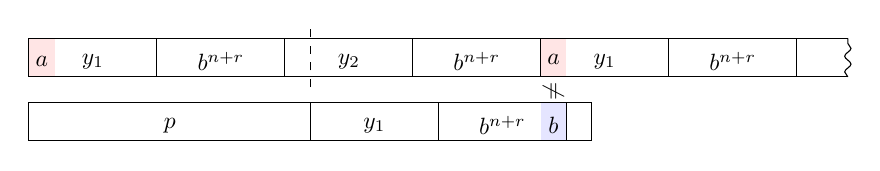
\begin{tikzpicture}[scale=0.65,every node/.style={scale=0.85}]
	\path[fill=red!10] (0,0) rectangle (0.5,0.75);
	\path[fill=blue!10] (10,-0.5) rectangle (10.5,-1.25);
	\path[fill=red!10] (10,0) rectangle (10.5,0.75);
	
	\draw (0,0) rectangle (15,0.75);
	\draw (15,0) -- (16,0);
	\draw[decorate,decoration={snake,amplitude=.4mm,segment length=2mm}] (16,0) -- (16,0.75);
	\draw (16,0.75) -- (15,0.75);
	
	\draw (2.5,0) -- (2.5,0.75);
	\draw (5,0) -- (5,0.75);
	\draw (7.5,0) -- (7.5,0.75);
	\draw (10,0) -- (10,0.75);
	\draw (12.5,0) -- (12.5,0.75);
	
	\node at (1.25,0.3) {$y_1$};
	\node at (3.75,0.3) {$b^{n+r}$};
	\node at (6.25,0.3) {$y_2$};
	\node at (8.75,0.3) {$b^{n+r}$};
	\node at (11.25,0.3) {$y_1$};
	\node at (13.75,0.3) {$b^{n+r}$};
	
	\draw[dashed] (5.5,-0.2) -- (5.5,0.95);
	
	\draw (0,-0.5) rectangle (5.5,-1.25);
	\draw (5.5,-0.5) rectangle (11,-1.25);
	\draw (8,-0.5) -- (8,-1.25);
	\draw (10.5,-0.5) -- (10.5,-1.25);
	
	\node at (2.75,-0.95) {$p$};
	\node at (6.75,-0.95) {$y_1$};
	\node at (9.25,-0.95) {$b^{n+r}$};
	
	\node at (0.25,0.3) {$a$};
	\node at (10.25,0.35) {$a$};
	\node at (10.25,-0.95) {$b$};
	
	\node[rotate=90] at (10.25,-0.275) {$\neq$};
\end{tikzpicture}